\documentclass[12pt]{article}
\usepackage{url,setspace,amsmath}
\usepackage{graphicx,xcolor}
\usepackage{fancyvrb}
% redefine \VerbatimInput
\RecustomVerbatimCommand{\VerbatimInput}{VerbatimInput}%
{fontsize=\footnotesize,}

\usepackage[letterpaper, left=0.9in, right=0.9in, top=0.9in, bottom=0.9in, nofoot, footnotesep=0.15in, headsep=0.15in, footskip=0.25in, nomarginpar]{geometry}

\begin{document}
\title{\vspace{-2cm}Documentation for dynamicNetwork: code for a dynamic network with fusion and fission}
\author{K.B.~Holt, E.~F.~Koslover}
\date{Last updated \today}
\maketitle

The code in this package will run a dynamic simulation of a network that is capable of fusion and fission. Each edge of the network is a straight segment between 2 nodes and represents (eg) a mitochondrial unit. Each node is an end-point of an edge (no lone nodes). Forces act on nodes. Fission happens at nodes of degree $> 1$. Fusion happens between degree-1 nodes or a degree-1 and a degree-2 node.

%\tableofcontents
%\newpage

\section{Compilation Instructions}
To compile and run the program, you will need the following:
\begin{itemize}
\item a compiler capable of handling Fortran90.
The code has been tested with the gfortran compiler.
\item Optionally: Matlab to visualize output data
\end{itemize}

The code has been tested on Ubuntu Linux 22.04.

\bigskip\noindent
To compile with gfortran, go into the \path=source= directory. Type \verb=make=.
To compile with any other compiler that can handle Fortran90, type
\begin{verbatim}
make FC=compiler
\end{verbatim}
substituting in the command you usually use to call the compiler.

\noindent
If the compilation works properly, the executable \path=dynnetwork.exe= will appear in the main directory.

\section{Usage Instructions}
To run the program in the main directory, type:
\begin{verbatim}
./dynnetwork.exe suffix > stdout.suffix
\end{verbatim}

Here, \verb=suffix= can be any string up to 100 characters in length.
The program reads in all input information from a file named
\path=param.suffix= where \verb=suffix= is the command-line
argument. If no argument is supplied, it will look for a file named
\path=param=. If the desired parameter file does not exist, the
program will exit with an error.

The parameters in the input file are given in the format "{\em KEYWORD} value" where the possible keywords and values are described
in Section \ref{sec:keywords}. Each keyword goes on a separate
line. Any line that starts with "\#" is treated as a comment and
ignored. Any blank line is also ignored. The keywords in the parameter
file are not case sensitive. For the most part, the order in which the
keywords are given does not matter. All parameters have default
values, so you need only specify keywords and values when you want to
change something from the default.


\section{Example for a Quick Start}
\subsection{Example 1}

A set of example parameter files (\verb=param.example_0_0_j=) are provided in the \verb=param_files= folder. Each parameter file will run a dynamic network simulation with 250 edges for $2\text{x}10^6$ simulation time steps and a different value of the fusion rate. To run the examples, navigate to the \verb=param_files= directory and run each example with
\begin{verbatim}
../dynnetwork.exe example_0_0_j > stdout.example_0_0_j
\end{verbatim}

If your machine has multiple processors, the simulations can be run in parallel. Snapshots of the network structure will be written to the file (\verb=example_0_0_j.snap.out=) every 1000 simulation steps. Each fusion and fission event will be recorded in the file (\verb=example_0_0_j.ffevents.out=). Use the script \verb=checkexample.m= (in the scripts folder) to visualize a given network structure over time, and the resulting plot of $\hat{\rho}C_2$ once all 10 simulations are finished. To run this script successfully, you must also add \verb=github.com/lenafabr/networktools/NetworkObj.m= to your path. The resulting visualizations should look something like this:

\centerline{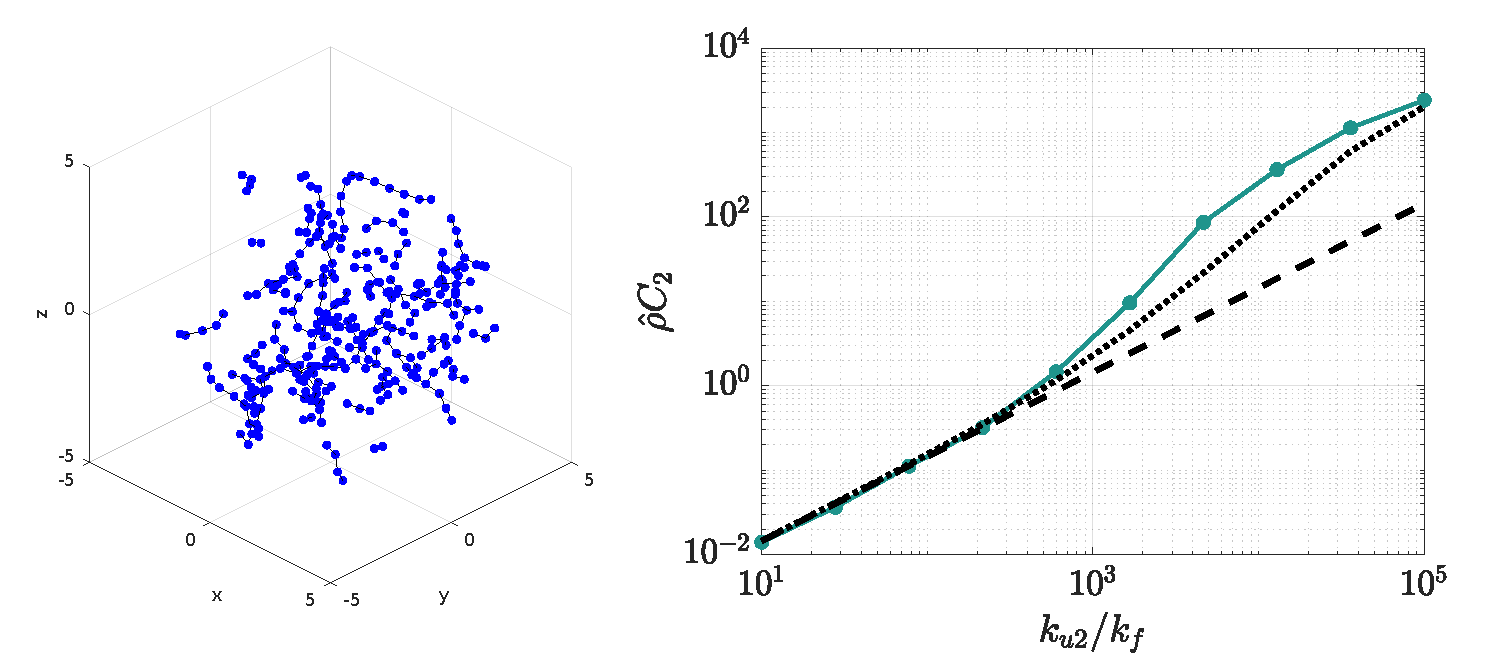
\includegraphics[width=0.9\textwidth]{example_panel.pdf}}

% ---------------------------------------------------------

\section{Keyword Index}
\label{sec:keywords}
The code will attempt to read parameters out of a file named \path=param.suffix= where ``suffix'' is the command line argument. If no command line arguments are supplied, it will look for a file named \path=param=. If multiple arguments are supplied, it will read multiple parameter files in sequence.

The parameter file should have one keyword per line and must end with a blank line. All blank lines and all lines beginning with \# are ignored. For the most part, the order of the lines and the capitalization of the keywords does not matter. All keywords except {\em ACTION} are optional. The default values for each parameter are listed below. If a keyword is supplied, then values may or may not be needed as well. Again, the required and optional value types are listed below.

Keywords and multiple values are separated by spaces.

When reading the parameter file, lines longer than 500 characters will be truncated. To continue onto the next line, add ``+++'' at the end of the line to be continued.
No individual keyword or  value should be longer than 100 characters.

Floating point numbers can be formated as $1.0$, $1.1D0$, $10e-1$, $-1.0E+01$, etc., where the exponential notation specifier must be D or E (case insensitive). Integer numbers can also be specified in exponential notation without decimal points (eg: 1000 or 1E3). Logical values can be specified as T, F, TRUE, FALSE, 1, or 0 (with 1 corresponding to true and 0 to false).


\subsubsection*{Simulation Setup}
\begin{itemize}
%
\item {\it ACTION}
  \begin{itemize}
    \item  value: 1 string of at most 20 characters; no default
    \item Possible values are: RUNDYNAMICS
  \end{itemize}
%
\item {\it BDSTEPS}
  \begin{itemize}
    \item  value: 1 integer; default 1000
    \item Number of Brownian dynamics steps to run
  \end{itemize}
%
\item {\it RNGSEED}
  \begin{itemize}
    \item 1 integer; default: $0$
    \item seed for random number generator
    \item value of 0 will seed with system time in milliseconds
    \item value of -1 will use the last 5 characters in the suffix
    \item value of -2 will use the last 4 charactes in the suffix and the millisecond time
    \item other positive value: the seed is used directly for repeatable simulations (should be positive)
    \item Negative values $< -2$: undefined, do not use (may give identical simulations or not; could be compiler dependent).
  \end{itemize}
%
\item {\it DIM}
  \begin{itemize}
    \item  value: 1 integer; default 3
    \item Dimensionality of the space in which the network is embedded
    \item Currently not set up for use in DIM $\ne$ 3
  \end{itemize}
%
\item {\it USEGRID}
  \begin{itemize}
    \item  value: 1 logical; default true
    \item Whether to use a spatial grid method to speed up pairwise distance calculations
  \end{itemize}
%
\item {\it USEEDGEGRID}
\begin{itemize}
  \item  value: 1 logical; default false
  \item Whether to use a spatial grid method to further speed up steric interaction calculations between edges. Requires USEGRID set to true
\end{itemize}
%
\item {\it USENODEGRID}
  \begin{itemize}
    \item  value: 1 logical; default false
    \item Whether to use a spatial grid method to speed up pairwise distance calculations for fusion between nodes. Requires USEGRID set to true
  \end{itemize}
%
\item {\it GRIDSPACES}
  \begin{itemize}
    \item  value: 1 or DIM integers; default 10
    \item Number of grid cubes in the spatial grid along each spatial dimension
  \end{itemize}
\end{itemize}

\subsubsection*{Mechanics}
\begin{itemize}
    %
\item {\it ESTR}
\begin{itemize}
  \item  value: 1 float; default 1000
  \item Stretch modulus for individual segments
\end{itemize}
%
\item {\it BENDMOD1}
\begin{itemize}
  \item  value: 1 float; default 2.0
  \item Bending modulus for degree 2 nodes. This value also sets the angular sensitivity for tip-tip fusion unless ALPHA1 is set
\end{itemize}
%
\item {\it BENDMOD2}
\begin{itemize}
  \item  value: 1 float; default 6.0
  \item Bending modulus for degree 3 nodes. This value also sets the angular sensitivity for tip-side fusion unless ALPHA2 is set
\end{itemize}
%
\item {\it THETA0}
\begin{itemize}
  \item  value: 1 float; default $\pi/3$
  \item Equilibrium "bond angle" for degree 3 nodes
\end{itemize}
%
\item {\it STERICMOD}
\begin{itemize}
  \item  value: 1 float; default 1D4
  \item Energy prefactor for steric interactions
\end{itemize}
%
\item {\it STERICRAD}
\begin{itemize}
  \item  value: 1 float; default 0.1
  \item Radius at which edges begin to sterically repel
\end{itemize}
  %
  \item {\it USEOUTOFPLANE}
    \begin{itemize}
      \item  value: 1 logical ; default: false
      \item Whether to incorporate an explicit out-of-plane bending energy term at degree-3 junctions (also used to define fusion rates).
    \end{itemize}
  %
  \item {\it BENDMODPLANE}
    \begin{itemize}
      \item  value: 1 float ; default: $0.6$
      \item  Bending stiffness prefactor for out-of-plane deviations at degree-3 junctions.
    \end{itemize}
  %
  \item {\it ALPHAPLANE}
    \begin{itemize}
      \item  value: 1 float; default $2\times$BENDMODPLANE
      \item Fusion sensitivity parameter for fusion between a degree-1 node and a degree-2 node corresponding to the out-of-plane energy.
    \end{itemize}
\end{itemize}
  
\subsubsection*{Fusion and Fission}
\begin{itemize}
%
\item {\it FISSRATE}
  \begin{itemize}
    \item  value: 1 float ; default: $0.0$
    \item Fission rate, per time, per fissable node (degree$>$1)
  \end{itemize}
%
%
\item {\it D3FISSMULT}
  \begin{itemize}
    \item  value: 1 float; default $1.5$
    \item The multiplier defining the likelihood of fission at degree-3 junctions relative to degree-2 junctions.
  \end{itemize}
%
\item {\it RECHARGERATE}
  \begin{itemize}
    \item  value: 1 float; default $-1.0$
    \item Rate at which nodes return to an active-fusion state following fission. Values less than zero will set this rate to $\infty$, meaning nodes are always allowed to re-fuse during the next time step after a fission event occurs.
  \end{itemize}
%
\item {\it FUSERATE1}
  \begin{itemize}
    \item  value: 1 float ; default: $0.0$
    \item Fusion rate, per time, per fuseable pair of degree-1 nodes
  \end{itemize}
%
\item {\it FUSERATE2}
\begin{itemize}
  \item  value: 1 float ; default: $0.0$
  \item Fusion rate, per time, per fuseable pair of degree-1, degree-2 nodes
\end{itemize}
%
\item {\it CONTACTRAD}
  \begin{itemize}
    \item  value: 1 float; default: $0.15$
    \item  Fusion is allowed when nodes are separated by a distance $2\times$CONTACTRAD or less.
  \end{itemize}
%
\item {\it ALPHA1}
\begin{itemize}
  \item  value: 1 float ; default: $2\times$BENDMOD1
  \item Fusion sensitivity parameter for fusion between degree-1 nodes
\end{itemize}
%
\item {\it ALPHA2}
\begin{itemize}
\item  value: 1 float ; default: $2\times$BENDMOD2
\item Fusion sensitivity parameter for fusion between a degree-1 and degree-2 node
\end{itemize}
\end{itemize}

\subsubsection*{Dynamics}
\begin{itemize}
%
\item {\it DELT}
  \begin{itemize}
    \item  value: 1 float; default 1D-4
    \item Time-step for the dynamics
  \end{itemize}
%
\item {\it FRICT}
  \begin{itemize}
    \item  value: 1 float; default: $1.0$
    \item Frictional coefficient for nodes
  \end{itemize}
%
\item {\it KT}
  \begin{itemize}
    \item  value: 1 float; default: $1.0$
    \item Temperature ($k_b T$) for Brownian dynamics
  \end{itemize}
\end{itemize}

\subsubsection*{Network and Boundary Setup}
\begin{itemize}
%
\item {\it MITOLEN}
  \begin{itemize}
    \item  value: 1 float; default: 0.5
    \item Ground-state edge length
  \end{itemize}
%
\item {\it MAXNEDGE}
  \begin{itemize}
    \item  value: 1 integer; default: $250$
    \item Maximum allowed number of edges in the network (code will exit with error if this is exceeded)
  \end{itemize}
%
\item {\it MAXNNODE}
  \begin{itemize}
    \item  value: 1 integer; default: $500$
    \item Maximum allowed number of nodes in the network (code will exit with error if this is exceeded). Safest to set MAXNNODE to $2\times$MAXNEDGE
  \end{itemize}
%
\item {\it USERANDOMFRAGMENTEDNETWORK}
\begin{itemize}
  \item  value: 1 logical; default: true
  \item Whether to start the simulation from a random network generated by placing isolated edges (all nodes will initially be degree-1) uniformly throughout the spherical volume
\end{itemize}
%
\item {\it NETFILE}
  \begin{itemize}
    \item  value: 1 string; default: *.net
    \item Input network file (full format with NODE lines, etc) used to start the simulation. If USEFRAGMENTEDNETWORK is set to true, this network file will not be used.
    \item Any * in the file name will be replaced by the command-line argument (suffix)
  \end{itemize}
%
\item {\it CONFSPHERE}
    \begin{itemize}
      \item  value: 1 to 2 floats; defaults: -1D0, 1D4
      \item CELLRAD1, ECONF (confinement radius, energy prefactor)
      \item Confine the network inside a sphere of radius CELLRAD1. The confinement energy is quadratic with prefactor ECONF. These two parameters may alternatively be specified on their own lines
\end{itemize}
%
\item {\it NPLANE}
  \begin{itemize}
    \item  value: 1 integer ; default: $0$
    \item If using planes to confine the network (rather than the default spherical boundary), the number of planes making up the boundary.
  \end{itemize}
%
\item {\it PLANEFILE}
  \begin{itemize}
    \item  value: 1 string; default: *.pl
    \item Input file used to build the planes defining the confining boundary of the network. NPLANE must match the number of planes specified in the file
    \item Any * in the file name will be replaced by the command-line argument (suffix)
  \end{itemize}
\end{itemize}

\subsubsection*{Outputting Data}
\begin{itemize}
%
\item {\it PRINTEVERY}
  \begin{itemize}
    \item  value: 1 integer; default: $1$
    \item Sets the step interval at which a status update should print to the screen
  \end{itemize}
%
\item {\it SNAPSHOTFILE}
  \begin{itemize}
    \item  value: 1 string; default: *.snap.out
    \item File for dumping out snapshots. Can also be specified within SNAPSHOTS keyword.
  \end{itemize}
%
\item {\it REMODELINGFILE}
  \begin{itemize}
    \item  value: 1 string; default: *.ffevents.out
    \item File for dumping out fission/fusion event records.
  \end{itemize}
%
\item {\it SNAPSHOTS}
  \begin{itemize}
    \item 1 optional integer, 1 optional string, 1 optional logical; defaults: 1, *.snap.out, false
    \item Dump snapshots over the course of the calculation
    \item integer: how often to dump snapshots; string: snapshot file (* is replaced with suffix); logical: append rather than rewriting the snapshot file
    \item Snapshot file contains multiple snapshots of network structure and other info. Should be read with \verb=parseDynNetworkSnapshots.m= script
  \end{itemize}
%
\item {\it STARTSNAPSTEP}
  \begin{itemize}
    \item  value: 1 integer; default: 1
    \item Simulation step to begin saving snapshots
  \end{itemize}

\item {\it VERBOSE}
  \begin{itemize}
    \item  value: 1 logical; default: false
    \item Print extra output.
  \end{itemize}
\end{itemize}

\subsubsection*{Yeast Model}
\begin{itemize}
%
\item {\it DOYEAST}
  \begin{itemize}
    \item  value: 1 logical; default false
    \item Whether to tether nodes to the cell boundary, creating a network geometry in which edges are constrained to the inner surface of a spherical shell.
  \end{itemize}
%
\item {\it YEASTCONF}
  \begin{itemize}
    \item  value: 1 float; default $100$
    \item The confinement energy tethering the nodes to the cell boundary is quadratic with prefactor YEASTCONF.
  \end{itemize}
%
\item {\it YEASTBINDRANGE}
  \begin{itemize}
    \item  value: 1 float; default 2.0
    \item Maximum distance from the cell boundary at which a node can become tethered.
  \end{itemize}
%
\item {\it YEASTONRATE}
  \begin{itemize}
    \item  value: 1 float; default 1.0
    \item Rate for each node to become tethered to the cell boundary when within YEASTBINDRANGE.
  \end{itemize}
%
\item {\it YEASTOFFRATE}
  \begin{itemize}
    \item  value: 1 float; default 1.0
    \item Rate for each node to fall off of the cell boundary when tethered.
  \end{itemize}
\end{itemize}
  
\subsubsection*{Diffusion on the Network}
\begin{itemize}
%
\item {\it NSPECIES}
  \begin{itemize}
    \item  value: 1 integer ; default: $0$
    \item Number of different types of particles to propagate along the network via diffusion (uses Finite-Volume-Method).
  \end{itemize}
%
\item {\it STARTDIFFSTEP}
  \begin{itemize}
    \item  value: 1 integer; default: 1
    \item Simulation step to begin propagating diffusing particles through the network.
  \end{itemize}
%
\item {\it DIFF}
  \begin{itemize}
    \item  value: NSPECIES floats ; default: 0.0
    \item Diffusion constant for each of the NSPECIES types of diffusing particles.
  \end{itemize}
%
\item {\it NSUBSTEPS}
  \begin{itemize}
    \item  value: 1 integer ; default: 0
    \item The number of steps which should be taken during the diffusion calculation for each timestep used by the rest of the simulation. (i.e. value 10 means a timestep of DELT/10 will be used to perform the diffusion calculation)
  \end{itemize}
%
\item {\it PRODRATE}
  \begin{itemize}
    \item  value: 1 or NSPECIES floats ; default: $-1.0$
    \item Rate at which new particles of each type are added to producing edges.
  \end{itemize}
%
\item {\it DECAYRATE}
  \begin{itemize}
    \item  value: 1 or NSPECIES floats; default $-1.0$
    \item Rate at which diffusing particles of each type decay on the network.
  \end{itemize}
%
\item {\it NUMTRIGGERUNITS}
  \begin{itemize}
    \item  value: 1 integer ; default: $0$
    \item The number of edges at which diffusing particles should be produced.
  \end{itemize}
%
\item {\it UNIQUETRIGGERS}
  \begin{itemize}
    \item  value: 1 logical ; default: false
    \item Whether to randomly select a unique set of producing edges for each type of diffusing particle, or use the same set for all types.
  \end{itemize}
%
\item {\it FIXEDGES}
  \begin{itemize}
    \item  value: 1 logical; default false
    \item Whether to hold the concentration of the set of producing edges at a fixed value of 1.
  \end{itemize}

\end{itemize}


\section{.net network file structure}
\label{sec:netfile}
Here is an example network file for use to begin a simulation from a pre-built network structure. Note that edge lengths need not be specified.
\VerbatimInput{example.net}

\section{.pl planes file structure}
\label{sec:planefile}
Here is an example planes file for use to begin a simulation in a non-spherical geometry. Each plane segment is specified as a vertex with (x,y,z) coordinates and two direction vectors. The magnitude of each direction vector sets the length of the plane in that direction. The plane will be ``oriented" in the direction given by the cross product of the unit vectors corresponding to the two direction vectors. Nodes which are ``below'' the plane (as defined by its orientation) will experience a force normal to the plane in the direction of its orientation.
\VerbatimInput{example.pl}


\end{document}
